\section{Data Challenges} \label{sec:data_challenges_extended}

In this section, we highlight some details that were omitted in section~\ref{sec:data_challenges}.
This includes details about the simulation type, the data structures, and the training/evaluation periods.

\subsection{OSSE NADIR}

The reference simulation is the \textit{NATL60} simulation based on the NEMO model~\cite{NEMOAJAYI2020}. 
This particular simulation was run over an entire year without any tidal forcing.
The simulation provides the outputs of SSH, SST, sea surface salinity (SSS) and the u,v velocities every 1 hour.
For the purposes of this data challenge, the spatial domain is over the Gulfstream with a spatial domain of $[-65^\circ, -55^\circ]$ longitude and $[33^\circ, 43^\circ]$ latitude.
The resolution of the original simulation is 1/60$^\circ$ resolution with hourly snapshots, and we consider a daily downsampled trajectory at 1/20$^\circ$ for the data challenge which results in a 365x200x200 spatio-temporal grid.
This simulation resolves finescale dynamical processes ($\sim$15km) which makes it a good test bed for creating an OSSE environment for mapping.
The SSH observations include simulations of ocean satellite NADIR tracks.
In particular, they are simulations of Topex-Poseidon, Jason 1, Geosat Follow-On, and Envisat.
There is no observation error considered within the challenge.
We use a the entire period from 2012-10-10 until 2013-09-30.
A training period is only from 2013-01-02 to 2013-09-30 where the users can use the reference simulation as well as all available simulated observations.
The evaluation period is from 2012-10-22 to 2012-12-02 (i.e. 41 days) which is considered decorrelated from the training period. 
During the evaluation period, the user cannot use the reference NATL60 simulation but they can use all available simulated observations. There is also a spin-up period allowance from 2012-10-01 where the user can also use all available simulated observations.

\subsection{OSSE SWOT \& OSSE SST}

For the OSSE SWOT and OSSE SST experiments, the reference simulation, domain, and evaluation period is the same as the OSSE NADIR experiment.
However, the OSSE SWOT includes simulated observations of the novel KaRIN sensor recently deployed during the SWOT mission, the pseudo-observations were generated using the SWOT simulator~\cite{SWOT}. 
This OSSE SST experiment allows the users to utilize the full fields of SST as inputs to help reconstruct the SSH field in conjunction with the NADIR and SWOT SSH observation.
Because the SST comes from the same NATL60 simulation, the geometry characteristics SST and SSH are exactly the same.

\subsection{OSE NADIR}

The OSE NADIR experiment only uses real observations aggregated from different altimeters. These SSH observations include observations from the SARAL/Altika, Jason 2, Jason 3, Sentinel 3A, Haiyang-2A and Cryosat-2 altimeters. The Cryosat-2 altimeter is used as the independent evaluation track used to assess the performance of the reconstructed SSH field.

\subsection{Results}

We use \texttt{OceanBench} to generate maps of relevant quantities from the 4DVarNet method~\cite{4DVARNETSWOT,4DVARNETSST}.
Figure~\ref{fig:oceanbench_maps_4dvarnet} showcases some demo maps for some key physical variables outlined in section~\ref{sec:physical_variables}.
We showcase the 4DVarNet method because it is the SOTA method that was applied to each of the data challenges.
We can see that the addition of more information, i.e. NADIR -> SWOT -> SST, results in maps look more similar to the NEMO simulation in the OSSE challenges.
It also produces sensible maps for the OSE challenge as well.

\texttt{OceanBench} also generated figure~\ref{fig:oceanbench_psd_4dvarnet} which shows plots of the PSD and PSD scores of SSH for the different challenges.
Again, as we increase the efficacy of the observations via SWOT and allow for more external factors like the SST, we get an improvement in the isotropic and spacetime PSD scores.
In addition, we see that the PSD plots for the OSE task look very similar to the OSE challenges. 

Lastly, we used \texttt{OceanBench} to generate a leaderboard of metrics for a diverse set of algorithms where the maps were available online.
Table~\ref{tb:exp-results-mega} displays all of the key metrics outlined in section~\ref{sec:metrics} including the normalized RMSE and various spectral scores which are appropriate for the challenge.
We see that as the complexity of the method increases, the metrics improve. 
In addition, the methods that involve end-to-end learning perform the best overall, i.e. 4DVarNet.

\begin{figure}[ht!]
\small
\begin{center}
\setlength{\tabcolsep}{1pt}
\begin{tabular}{cccc}
\hspace{3mm} Task OSSE & 
\hspace{3mm} Task OSSE & 
\hspace{2mm} Task OSSE & 
Task OSE \\
\hspace{3mm}  Nadir & 
\hspace{3mm} Nadir + SWOT & 
\hspace{2mm} Nadir + SST & 
Nadir \\
%\vspace{-2mm}
%%%%% SSH %%%%%%%%
\includegraphics[trim={0 13mm 22mm 0},clip, width=3.60cm,height=3.2cm]{00_Oceanbench/content/figures/fourdvarnet_figs/osse_gf_nadir_ssh.png} &
\includegraphics[trim={13mm 13mm 22mm 0},clip, width=3.2cm,height=3.2cm]{00_Oceanbench/content/figures/fourdvarnet_figs/osse_gf_nadirswot_ssh.png} &
\includegraphics[trim={13mm 13mm 22mm 0},clip, width=3.2cm,height=3.2cm]{00_Oceanbench/content/figures/fourdvarnet_figs/osse_gf_nadir_sst_ssh.png} &
\includegraphics[trim={13mm 13mm 0 0},clip,width=4.0cm,height=3.2cm]{00_Oceanbench/content/figures/fourdvarnet_figs/ose_gf_ssh.png} \\
%\vspace{3mm}
%%%%% KINETIC ENERGY %%%%%%%%
\includegraphics[trim={0 13mm 22mm 5mm}, clip, width=3.60cm,height=3cm]{00_Oceanbench/content/figures/fourdvarnet_figs/osse_gf_nadir_ke.png} &
\includegraphics[trim={13mm 13mm 22mm 5mm},clip, width=3.2cm,height=3cm]{00_Oceanbench/content/figures/fourdvarnet_figs/osse_gf_nadirswot_ke.png} &
\includegraphics[trim={13mm 13mm 22mm 5mm},clip, width=3.2cm,height=3cm]{00_Oceanbench/content/figures/fourdvarnet_figs/osse_gf_nadir_sst_ke.png} &
\includegraphics[trim={13mm 13mm 0 5mm},clip,width=4cm,height=3cm]{00_Oceanbench/content/figures/fourdvarnet_figs/ose_gf_ke.png} \\
%%%%% RELATIVE VORTICITY %%%%%%%%
\includegraphics[trim={0 13mm 21.2mm 5mm},clip, width=3.60cm,height=3cm]{00_Oceanbench/content/figures/fourdvarnet_figs/osse_gf_nadir_vort_r.png} &
\includegraphics[trim={13mm 13mm 21.2mm 5mm},clip, width=3.2cm,height=3cm]{00_Oceanbench/content/figures/fourdvarnet_figs/osse_gf_nadirswot_vort_r.png} &
\includegraphics[trim={13mm 13mm 21.2mm 5mm},clip, width=3.2cm,height=3cm]{00_Oceanbench/content/figures/fourdvarnet_figs/osse_gf_nadir_sst_vort_r.png} &
\includegraphics[trim={13mm 13mm 0 5mm},clip,width=4.0cm,height=3cm]{00_Oceanbench/content/figures/fourdvarnet_figs/ose_gf_vort_r.png} \\
%%%%% STRAIN %%%%%%%%
\includegraphics[trim={0 0 19mm 5mm},clip, width=3.60cm,height=3.4cm]{00_Oceanbench/content/figures/fourdvarnet_figs/osse_gf_nadir_strain.png} &
\includegraphics[trim={13mm 0 19mm 5mm},clip, width=3.2cm,height=3.4cm]{00_Oceanbench/content/figures/fourdvarnet_figs/osse_gf_nadirswot_strain.png} &
\includegraphics[trim={13mm 0 19mm 5mm},clip, width=3.2cm,height=3.4cm]{00_Oceanbench/content/figures/fourdvarnet_figs/osse_gf_nadir_sst_strain.png} &
\includegraphics[trim={13mm 0 0 5mm},clip,width=4.0cm,height=3.4cm]{00_Oceanbench/content/figures/fourdvarnet_figs/ose_gf_strain.png} \\
% \vspace{-2mm}
(a) & (b) & (c) & (d)
\end{tabular}
\vspace{-3mm}
% \caption{Row I - Isotrophic PSD. Row 2 - Isotrophic PSD Score}
\caption{
Reconstructed quantities by the 4dVarNet method for each of the four tasks.
Each row showcases the following physical variables found in appendix~\ref{sec:physical_variables}: (a) Sea Surface Height, (b) Kinetic Energy, (c) Relative Vorticity, and (d) Strain. 
Each column showcase the reconstructed from the tasks (a) OSSE using only Nadir tracks: (b) OSSE using Nadir tracks and SWOT swath, (c) Multimodal using Nadir tracks and sea surface temperature, and (d) Reconstruction using real nadir altimetry tracks.}
\vspace{-5mm}
\label{fig:oceanbench_maps_4dvarnet}
\end{center}
\end{figure}





% \begin{figure}[ht!]
\small
\begin{center}
\setlength{\tabcolsep}{1pt}
\begin{tabular}{cccc}
\hspace{3mm} Task OSSE & 
\hspace{3mm} Task OSSE & 
\hspace{2mm} Task OSSE & 
Task OSE \\
\hspace{3mm}  Nadir & 
\hspace{3mm} Nadir + SWOT & 
\hspace{2mm} Nadir + SST & 
Nadir \\
%\vspace{-2mm}
%%%%% SSH %%%%%%%%
\includegraphics[trim={0 13mm 22mm 0},clip, width=3.60cm,height=3.2cm]{content/figures/fourdvarnet_figs/osse_gf_nadir_ssh.png} &
\includegraphics[trim={13mm 13mm 22mm 0},clip, width=3.2cm,height=3.2cm]{content/figures/fourdvarnet_figs/osse_gf_nadirswot_ssh.png} &
\includegraphics[trim={13mm 13mm 22mm 0},clip, width=3.2cm,height=3.2cm]{content/figures/fourdvarnet_figs/osse_gf_nadir_sst_ssh.png} &
\includegraphics[trim={13mm 13mm 0 0},clip,width=4.0cm,height=3.2cm]{content/figures/fourdvarnet_figs/ose_gf_ssh.png} \\
%\vspace{3mm}
%%%%% KINETIC ENERGY %%%%%%%%
\includegraphics[trim={0 13mm 22mm 5mm}, clip, width=3.60cm,height=3cm]{content/figures/fourdvarnet_figs/osse_gf_nadir_ke.png} &
\includegraphics[trim={13mm 13mm 22mm 5mm},clip, width=3.2cm,height=3cm]{content/figures/fourdvarnet_figs/osse_gf_nadirswot_ke.png} &
\includegraphics[trim={13mm 13mm 22mm 5mm},clip, width=3.2cm,height=3cm]{content/figures/fourdvarnet_figs/osse_gf_nadir_sst_ke.png} &
\includegraphics[trim={13mm 13mm 0 5mm},clip,width=4cm,height=3cm]{content/figures/fourdvarnet_figs/ose_gf_ke.png} \\
%%%%% RELATIVE VORTICITY %%%%%%%%
\includegraphics[trim={0 13mm 21.2mm 5mm},clip, width=3.60cm,height=3cm]{content/figures/fourdvarnet_figs/osse_gf_nadir_vort_r.png} &
\includegraphics[trim={13mm 13mm 21.2mm 5mm},clip, width=3.2cm,height=3cm]{content/figures/fourdvarnet_figs/osse_gf_nadirswot_vort_r.png} &
\includegraphics[trim={13mm 13mm 21.2mm 5mm},clip, width=3.2cm,height=3cm]{content/figures/fourdvarnet_figs/osse_gf_nadir_sst_vort_r.png} &
\includegraphics[trim={13mm 13mm 0 5mm},clip,width=4.0cm,height=3cm]{content/figures/fourdvarnet_figs/ose_gf_vort_r.png} \\
%%%%% STRAIN %%%%%%%%
\includegraphics[trim={0 0 19mm 5mm},clip, width=3.60cm,height=3.4cm]{content/figures/fourdvarnet_figs/osse_gf_nadir_strain.png} &
\includegraphics[trim={13mm 0 19mm 5mm},clip, width=3.2cm,height=3.4cm]{content/figures/fourdvarnet_figs/osse_gf_nadirswot_strain.png} &
\includegraphics[trim={13mm 0 19mm 5mm},clip, width=3.2cm,height=3.4cm]{content/figures/fourdvarnet_figs/osse_gf_nadir_sst_strain.png} &
\includegraphics[trim={13mm 0 0 5mm},clip,width=4.0cm,height=3.4cm]{content/figures/fourdvarnet_figs/ose_gf_strain.png} \\
% \vspace{-2mm}
(a) & (b) & (c) & (d)
\end{tabular}
\vspace{-3mm}
% \caption{Row I - Isotrophic PSD. Row 2 - Isotrophic PSD Score}
\caption{
Reconstructed quantities by the 4dVarNet method for each of the four tasks.
Each row showcases the following physical variables found in appendix~\ref{sec:physical_variables}: (a) Sea Surface Height, (b) Kinetic Energy, (c) Relative Vorticity, and (d) Strain. 
Each column showcase the reconstructed from the tasks (a) OSSE using only Nadir tracks: (b) OSSE using Nadir tracks and SWOT swath, (c) Multimodal using Nadir tracks and sea surface temperature, and (d) Reconstruction using real nadir altimetry tracks.}
\vspace{-5mm}
\label{fig:oceanbench_maps_4dvarnet}
\end{center}
\end{figure}


\begin{table}[ht]
\caption{This table showcases all of the summary statistics for some methods for each of the data challenges listed in section~\ref{sec:data_challenges} and~\ref{sec:data_challenges_extended}. The summary statistics shown are the normalized RMSE and the effective resolution in the spectral domain. The spectral metrics for the effective resolution that were outlined in section~\ref{sec:metrics} are: i) $\lambda_a$ is the spatial score for the alongtrack PSD score, ii) $\lambda_r$ is the spatial score for the isotropic PSD, iii) $\lambda_x$ is the spatial score for space-time PSD score, and iv) $\lambda_t$ is the temporal score for the space-time PSD score.}
% \caption{This table highlights some of the results for the OSSE experiments outlined in section~\ref{sec:osse} and~\ref{sec:other_tasks}.

% This table highlights the performance statistically in the real and spectral space; the normalized RMSE for the real space and the minimum spatial and temporal scales resolved in the spectral domain. 
% For more information about the class of models displayed and class of metrics, see section~\ref{sec:ml_ontology} and section~\ref{sec:metrics} respectively.}
\label{tb:exp-results-mega}
\centering
\begin{tabular}{llcccccc}
 \toprule
% Experiment & Configuration & Method & nRMSE & Resolved Scale [km]    \\ \midrule
% \multirow{2}{*}{Experiment} & \multirow{2}{*}{Algorithm} & \multirow{2}{*}{Algorithm Class} & \multirow{2}{*}{nRMSE} & \multicolumn{2}{c}{Effective Resolution} \\ 
% &  &   &  & Wavelength [km]  & Period [days]      \\ \midrule
% \multirow{2}{*}{Experiment} & \multirow{2}{*}{Algorithm} & \multirow{2}{*}{Algorithm Class} & \multirow{2}{*}{nRMSE} & \multicolumn{2}{c}{Effective Resolution} \\ 
\multirow{2}{*}{Experiment} &  \multirow{2}{*}{Algorithm} &   \multirow{2}{*}{nRMSE} &
\multicolumn{4}{c}{Effective Resolution} \\
& & & $\lambda_{a}$ [km] & $\lambda_{r}$ [km]   &  $\lambda_{\mathbf{x}}$ [km]  &   $\lambda_{t}$ [days]      \\ \midrule
OSSE NADIR     &  OI & 0.92 & - & 123 & 174 & 10.8 \\
OSSE NADIR     &  MIOST &  0.93 & - & 100 & 157 & 10.1 \\
OSSE NADIR     &  BFNQG & 0.93 & - & 88 & 139 & 10.4 \\
OSSE NADIR &  4DVarNet &  \textbf{0.94} & - & \textbf{65} & \textbf{117} & \textbf{7.7} \\
\midrule
OSSE SWOT     &  OI & 0.92 & - & 106 & 139 & 11.7 \\
OSSE SWOT     &  MIOST &  0.94 & - & 88 & 131 & 10.1 \\
OSSE SWOT     &  BFNQG & 0.94 & - & 64 & 118 & 36.5 \\
OSSE SWOT &  4DVarNet &  \textbf{0.96} & - & \textbf{47} & \textbf{77} & \textbf{5.6} \\
\midrule
OSSE SST     &  Musti & 0.95 & - & 46 & 138 & 4.1 \\
OSSE SST &  4DVarNet &  \textbf{0.96} & - & \textbf{46} & \textbf{87} & \textbf{3.7} \\
\midrule
OSE NADIR     &  OI & 0.88 & 151 & - &  - &  -\\
OSE NADIR     &  MIOST &  0.90 & 135 & - &  - &  -\\
OSE NADIR     &  BFNQG & 0.88 & 122 & - & - &  -\\
OSE NADIR &  ConvLSTM &  0.89 & 113 &- &  - &  -\\
OSE NADIR &  4DVarNet & \textbf{0.91} & \textbf{98} & - &  -  &  -\\
\bottomrule
\end{tabular}
\end{table}

% \subsection{Simulated Altimetry Tracks} \label{sec:dc_osse_nadir}

% \textcolor{red}{
% The most commonly used SSH maps, the Developing Use of Altimetry for Climate Studies (DUACS) products, are derived from a statistical space–time interpolation of nadir altimeter observations. This intrinsically limits the effective resolution [as defined in Skamarock (2004), i.e., the fully resolved scales] of DUACS SSH maps to 150–200 km at middle latitudes (Ballarotta et al. 2019). The SSH mapping algorithm was developed by CNES and CLS in 1997, as part of the DUACS project, and has been continuously improved since then (Taburet et al. 2019). The DUACS products are now distributed by the Copernicus Marine Environment Monitoring Service (CMEMS). DUACS algorithm implements a statistical interpolation of SSH satellite data in space and time to produce global daily maps (Le Traon et al. 1998). The data are collected by a constellation of 2 to 4 nadir-looking altimeters (sometimes referred to as conventional altimeters), and characterized by large data gaps reaching 200 km in the zonal direction at the equator.
% }

% \subsection{Simulated SWOT Tracks} \label{sec:dc_osse_swot}


% \textcolor{red}{
% The Surface Water and Ocean Topography (SWOT; Fu et al. 2012; Morrow et al. 2019) altimetry mission, to be launched in early 2022, will open the way to SSH maps with resolution significantly higher than 150 km at midlatitudes, but this perspective entails a thorough revisit of the mapping algorithm. SWOT will considerably increase the measurement density at the surface of the oceans thanks to SSH measurements at a kilometric pixel resolution over a swath 120 km wide. On the swath, SWOT is expected to resolve scales down to 15 km at low latitude and 30–45 km at mid- and high latitudes (Wang et al. 2019). In its science phase, SWOT will have a 21 days repeat orbit, allowing an average revisit time of 11 days in most of the globe. Some of the dynamical processes observable by SWOT evolve over time scales on the order of 1 day, much shorter than the satellite revisit time. Consequently, the mapping method implemented in the current DUACS system will certainly not be sufficient to draw the maximum benefit from SWOT. A linear interpolation will filter most of the observed small-scale signals between two passes of the satellite, as anticipated by Gaultier et al. (2016).These authors advocate for using more advanced methods to build SSH maps.
% }

% \subsection{Multimodal with Sea Surface Temperature}  \label{sec:dc_osse_sst}


% \subsection{Real Altimetry Tracks}  \label{sec:dc_ose_nadir}